% CAP 4 Poros. ecuaciones, como se resuelve, resultados
\chapter{Generación y Evolución de Poros} \label{chap:poros}

En este capítulo se simula la creación de poros en la membrana celular según las ecuaciones \ref{eq:poros-crea} y \ref{eq:poros-radio}. Para eso se utiliza el cálculo del potencial eléctrico realizado en el capítulo anterior, pero se le agrega la ecuación \ref{eq:capacit}, que tiene en cuenta la capacitancia de la célula al momento de calcular el potencial transmembrana y se actualizan los valores de conductividad en la membrana según la permeabilización lograda por los poros.

\section{Implementación}

Como las ecuaciones que gobiernan la creación de poros en la membrana son dependientes del tiempo, fue necesario crear un ciclo que realice iteraciones de las ecuaciones de poros y de potencial eléctrico. La ecuación \ref{eq:poisson} debe correrse periódicamente a pesar de que no depende del tiempo, ya que los valores de conductancias en la membrana ($\sigma_{m}$) son afectados por la aparición de poros. Las ecuaciones \ref{eq:poros-crea} y \ref{eq:poros-radio} fueron discretizadas con el método de Euler a un paso\footnote{Si se tiene una ecuación diferencial ordinaria tal que $Y'(x) = f(x, Y(x))$ y $Y(x_0) = Y_0$, el método de Euler con un paso $h$ aproxima la función $Y$ como $y_0 = Y_0$ y $y_{n+1} = y_n + h\,f(x_n, y_n)$ \cite{kendall}}.

La ecuación \ref{eq:poros-crea} que calcula la densidad de poros en cada región de la membrana fue discretizada como

%TODO esquema implícito, explícito etc!!!

\begin{equation} \label{eq:poros-crea-disc}
	\frac{N_{t+1} - N_{t}}{\Delta t} = \alpha e^{(V_m/V_{ep})^2} \left( 1 - \frac{N_{t}}{N_0 e^{q \left(V_m / V_{ep} \right) ^2}} \right)
\end{equation}

Para obtener el valor de $V_m$ en cada punto de la membrana celular se tienen en cuenta los potenciales obtenidos con el método de elementos finitos y la capacitancia de la célula. Primero se calcula la diferencia de potencial entre los nodos externos e internos de la membrana y luego se aplica la ecuación \ref{eq:capacit} para obtener el PTM real según el tiempo transcurrido desde el comienzo del pulso.

La cantidad de poros en cada región de la membrana se calcula multiplicando la densidad obtenida con la ecuación \ref{eq:poros-crea-disc} por el área de cada región discreta y tomando la parte entera del valor obtenido. El área de cada zona esférica discreta se calcula como 

\begin{equation} \label{eq:area}
	A = 2 \pi \alpha^2 (\cos(\theta_1) - \cos(\theta_2))
\end{equation}

siendo $\alpha$ el radio de la célula y $\theta_1$ y $\theta_2$ los ángulos que delimitan la zona esférica.

Se mantiene para cada zona esférica discreta un vector con cada uno de los poros y sus radios. Si en una iteración la cantidad de poros estimada para una región es mayor a cantidad de poros estimada en la iteración anterior, entonces se agregan poros al vector de la región esférica con radio inicial $r_*$.

Para cada uno de los poros se calcula por separado su radio en cada iteración aplicando la ecuación \ref{eq:poros-radio} discretizada como

\begin{equation} \label{eq:poros-radio-disc}
	\frac{r_{t+1} - r_t}{\Delta t} = \frac{D}{kT} \left( \frac{V_m^2 F_{max}}{1+r_h / (r_t+r_a)} + \frac{4 \beta}{r_t} \left(\frac{r_*}{r_t}\right)^4 - 2 \pi \gamma + 2 \pi \sigma_{\textrm{\tiny eff}} r_t \right)
\end{equation}

Para mejorar los tiempos de ejecución se consideran todos los poros con radio muy pequeño y con cierta antigüedad como iguales en vez de tratarlos individualmente, mientras que a los poros grandes o recién creados se los trata individualmente, aplicando la ecuación \ref{eq:poros-radio-disc} a cada uno, técnica utilizada en \cite{krass07}.

Los valores de conductividad de la membrana son afectados por la aparición de poros. Por esta razón se calcula primero la permeablización de cada región de la membrana como la proporción del área ocupada por poros con la fórmula

\begin{equation} 
    p = \frac{ \sum\limits_{r \in R} \pi r^2 }{A_z}
\end{equation} 

donde $p$ es la permeabilización de una zona esférica de la membrana, $R$ un conjunto con todos los radios de los poros en ésa zona y $A_z$ el área de la zona, calculada según la ecuación \ref{eq:area}. Luego se actualizan los valores de conductividad de cada zona de la membrana como

\begin{equation} 
	\sigma_{\textrm{\tiny elem}} = \sigma_m (1 - p) + \sigma_p p
\end{equation} 

con $\sigma_{\textrm{\tiny elem}}$ la nueva conductividad del elemento finito, $\sigma_m$ la conductividad de la membrana cuando no tiene poros y $\sigma_p$ la conductividad del líquido que llena los poros.

De la misma manera se actualizan los valores de difusión para los elementos de la membrana 

\begin{equation} 
	D{\textrm{\tiny elem}} = D_m (1 - p) + D_p p
\end{equation} 

con $D_m$ la difusión de la membrana celular sin poros y $D_p$ la difusión del líquido que llena los poros. Este cambio en la difusión no tiene por el momento ningún efecto pero lo tendrá en capítulos posteriores cuando se calcule el transporte de especies.

\section{Resultados}

Se corrieron simulaciones con células de 25\um de radio y pulsos de entre 1200\vcm y 1600\vcm y 5 \ms de duración. 

%acá poner histogramas de poros en diferentes instantes. Al menos para dos valores de tensión
%
%4 histogramas en total, para dos valores de tensión

\dobleimagengrandedonde{poros/120kvm/20micro}{histo-120-1}{Distribución de radios de los poros grandes \\ para $E = 1200\,\vcm$ en $t = 20\,\usec$}{poros/120kvm/500micro}{histo-120-2}{Distribución de radios de los poros grandes\\ para $E = 1200\,\vcm$ en $t = 500\,\usec$}{p}

\dobleimagengrandedonde{poros/160kvm/20micro}{histo-160-1}{Distribución de radios de los poros grandes\\ para $E = 1600\,\vcm$ en $t = 20\,\usec$}{poros/160kvm/500micro}{histo-160-2}{Distribución de radios de los poros grandes\\ para $E = 1600\,\vcm$ en $t = 500\,\usec$}{p}

En las figuras \ref{fig:histo-120-1} y \ref{fig:histo-120-2} se presentan histogramas con los radios de los poros grandes creados en diferentes instantes para pulsos de 1200 \si{\kilo\volt\per\centi\metre}. También hay una gran población de poros pequeños (con radio menor a 1 \si{\nano\metre}) que no fueron graficados por ser de poco interés. Se puede observar que la población de poros alcanza valores altos en un primer instante, pero se reduce dramáticamente en los instantes posteriores. En las figuras \ref{fig:histo-160-1} y \ref{fig:histo-160-2} se observa distribución de radios para la misma célula pero con un pulso de 1600 \si{\kilo\volt\per\centi\metre}. Tanto la cantidad como el radio de los poros creados es mayor en el segundo caso, y se observa también una disminución en la población pasados los primeros instantes del pulso. Es importante notar que si bien la cantidad de poros disminuye con el tiempo, los poros que quedan tienen un radio promedio notablemente mayor al de los primeros instantes.

\begin{figure}
	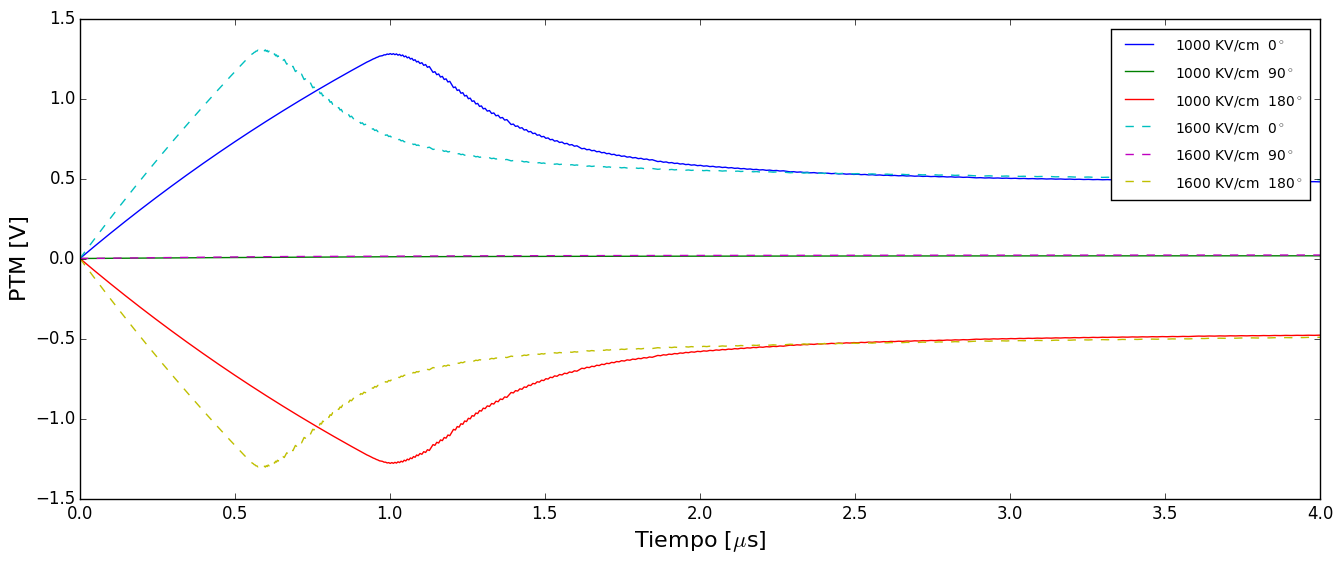
\includegraphics[width=\linewidth]{poros/itv-time}
	\caption{PTM en función del tiempo en distintos ángulos polares para dos potenciales aplicados diferentes}
	\label{fig:itv-time}
\end{figure}

%Se puede observar en la figura \ref{fig:itv-time} el potencial transmembrana en función del tiempo al comienzo del pulso para diferente ángulos polares $\theta$. Las cuatro figuras corresponden a cuatro pulsos de diferente potencial eléctrico aplicado sobre la misma célula. En el primer caso el potencial eléctrico es muy chico y por lo tanto no se alcanzaron a crear poros. En los otros casos el potencial sí es lo suficientemente alto como para crear poros. Se observa en estos casos que el PTM se incrementa durante los primeros instantes hasta alcanzar un pico de tensión a partir del cual comienza a disminuir hasta alcanzar un valor de equilibrio. La subida paulatina de tensión durante los primeros instantes del pulso se debe a la capacitancia de la célula, mientras que la caída en los instantes posteriores se debe a la aparición de poros, que disminuyen la conductividad de la membrana, disminuyendo de esta manera la caída de tensión entre el interior y exterior de la célula. 

%Se nota en todos los casos que las regiones de la membrana cercanas a los polos (con ángulos cercanos a 0º o 180º) obtienen en los primeros instantes los valores absolutos de PTM más altos, mientras que las regiones cercanas al ecuador (ángulo polar cercano a 90º) tienen un PTM prácticamente nulo.

Se puede observar en la figura \ref{fig:itv-time} el potencial transmembrana en función del tiempo al comienzo del pulso para diferentes ángulos polares $\theta$, con dos campos eléctricos diferentes. El PTM se incrementa durante los primeros instantes hasta alcanzar un pico de tensión a partir del cual comienza a disminuir hasta alcanzar un valor de equilibrio. La subida paulatina de tensión durante los primeros instantes del pulso se debe a la capacitancia de la célula, mientras que la caída en los instantes posteriores se debe a la aparición de poros, que disminuyen la conductividad de la membrana, disminuyendo de esta manera la caída de tensión entre el interior y exterior de la célula. Se nota que el PTM obtenido depende notablemente del ángulo polar: en la región polar cercana al electrodo positivo el PTM es positivo y alcanza valores altos, mientras que en el polo cercano al cátodo el potencial es negativo y en el ecuador es cercano a cero. Es llamativo que los valores de campo eléctrico aplicado no influyen en el valor de pico de PTM obtenido, pero si en el tiempo en que éste se alcanza; al aumentar el campo de 1000\vcm a 1600\vcm se acelera el proceso de subida y bajada de PTM hasta alcanzar un equilibrio, pero no se logran aumentar los potenciales obtenidos.


%aca poner gráficos de PTM vs ángulo para diff tiempos. estaría bueno poner una sola curva por gráfico y gráficos más chicos. podrian ser todos de un solo potencial en vez de diferentes tensiones

\dobleimagengrande{poros/120kvm/tita}{tita120}{PTM en función del ángulo polar\\ con $E = 1200\,\vcm$}{poros/160kvm/tita}{tita160}{PTM en función del ángulo polar\\ con $E = 1600\,\vcm$}

En las figuras \ref{fig:tita120} y \ref{fig:tita160} se graficaron los potenciales transmembrana en función del ángulo polar para diferentes instantes de tiempo con pulsos de potenciales diferentes en los dos gráficos. Se observa en los primeros instantes que el PTM obtenido es similar al obtenido en el capítulo anterior y al que se puede estimar con la fórmula cerrada \ref{eq:cos}. Esto se debe a que la población de poros es nula o muy pequeña como para afectar aún la conductividad de la membrana. Sin embargo en los instantes posteriores la aparición de poros disminuye notablemente la conductividad de la membrana en las regiones cercanas a los polos, bajando así la diferencia de potencial. En instantes posteriores se observa el mismo fenómeno con regiones más lejanas a los poros, alejándose más el PTM obtenido del que se puede calcular con la fórmula cerrada \ref{eq:cos}.\\

%%%%

Se estudió también el efecto de aplicar una señal de varios pulsos en lugar uno solo. En la figura \ref{fig:poros-tiempo} se graficó la cantidad de poros en función del tiempo para 4 pulsos de 5\ms de \ontime{} y 5\ms de \offtime{} con varios potenciales diferentes. Se puede ver que la cantidad de poros crece únicamente al principio de cada pulso, y se mantiene casi constante durante el resto del pulso, disminuyendo muy levemente durante el tiempo de apagado. Por cada pulso nuevo se crean poros nuevos, aunque la cantidad de poros nuevos disminuye con cada pulso consecutivo. Se puede ver también que el efecto del campo eléctrico sobre la densidad es enorme, obteniéndose poblaciones de casi el doble de poros para al aumentar el potencial aplicado de 1200\vcm a 1600 \si{\volt\per\centi\metre}. El valor de 500\vcm podría tomarse como el valor mínimo necesario para obtener una cantidad considerable de poros, mientras que para 400\vcm y otros valores menores la densidad es despreciable, es decir casi no se produce electroporación. 

En la figura \ref{fig:radios-tiempo} se graficó el promedio de los radios de los poros en función del tiempo. Se nota que los radios altos se obtienen por un instante muy corto de tiempo al principio de cada pulso, y que rápidamente se achican llegando a un valor de equilibrio en aproximadamente la mitad del tiempo del \ontime. Cuando el pulso se apaga, los radios se hacen rápidamente mínimos, y se mantienen en un valor muy chico hasta el inicio del próximo pulso. A diferencia de la cantidad de poros, el radio promedio disminuye al aumentar el potencial eléctrico. Esto puede deberse a que un mayor campo eléctrico produce muchos poros de radio mínimo, afectando el promedio de manera negativa. En cada pulso consecutivo parecen aumentar ligeramente los radios obtenidos, notándose la mayor diferencia entre los radios del primer y el segundo pulso. 

En las figuras \ref{fig:pulso1} a \ref{fig:pulso4} se observan las distribuciones de radios de poros para 1600\vcm al instante de 100\usec luego del comienzo de cada pulso. Las diferencias entre radios se observan sobre todo entre el primer y segundo pulso, mientras que los siguientes parecen tener distribuciones muy similares. La mayor concentración se encuentra siempre en los radios muy pequeños (de aproximadamente 1 \si{\nano\metre}), que afectan poco al proceso de permeabilización de la membrana.



\imagensola{poros/poros-tiempo}{poros-tiempo}{Cantidad de poros en función del tiempo para cuatro pulsos}{}
\imagensola{poros/radios-tiempo}{radios-tiempo}{Radio promedio de los poros en función del tiempo para cuatro pulsos}{}



%En las figuras \ref{pulso1} a \ref{pulso4} se observan las distribuciones de radios de poros para cuatro pulsos consecutivos. Los pulsos son de 160\kvcm con 5\ms de \ontime{} y 5\ms de \offtime{} y los histogramas corresponden al instante de 100\usec luego de comenzado cada pulso. \todo[inline]{escribir más después de poner cant poros vs tiempo}

%\dobleimagengrande{poros/160kvm/pulso1}{pulso1}{Primer pulso}{poros/160kvm/pulso2}{pulso2}{Segundo pulso}
%\dobleimagengrande{poros/160kvm/pulso3}{pulso3}{Tercer pulso}{poros/160kvm/pulso4}{pulso4}{Cuarto pulso}

\begin{figure} [ht!]
\makebox[\textwidth][c] {
	\centering
	\begin{minipage}{.43\paperwidth}
		\centering
		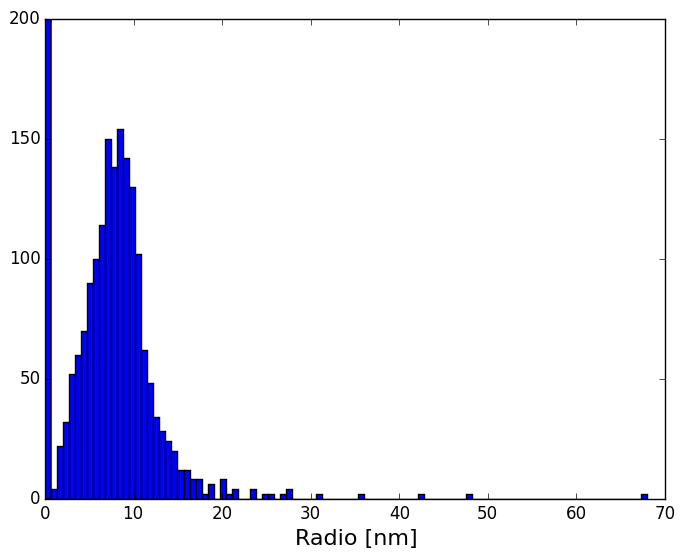
\includegraphics[width=1\linewidth]{poros/160kvm/pulso1}
		\captionof{figure}{Primer pulso}
		\label{fig:pulso1}
	\end{minipage}%
	\begin{minipage}{.43\paperwidth}
		\centering
		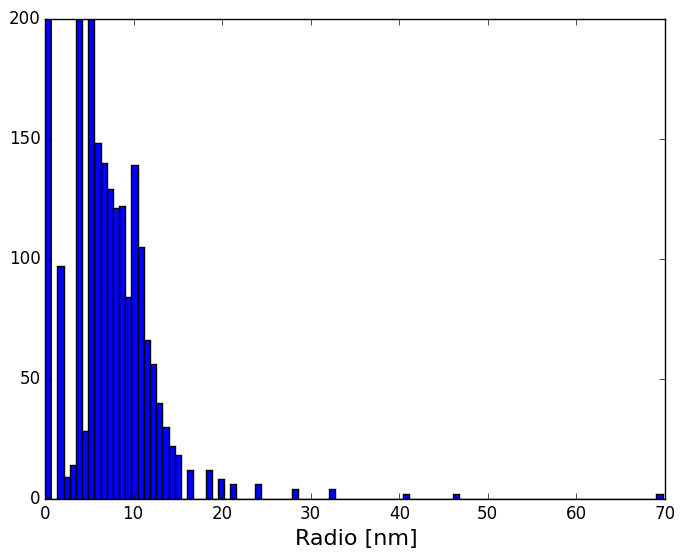
\includegraphics[width=1\linewidth]{poros/160kvm/pulso2}
		\captionof{figure}{Segundo pulso}
		\label{fig:pulso2}
	\end{minipage}
}
\end{figure}

\begin{figure} [ht!]
\makebox[\textwidth][c] {
	\centering
	\begin{minipage}{.43\paperwidth}
		\centering
		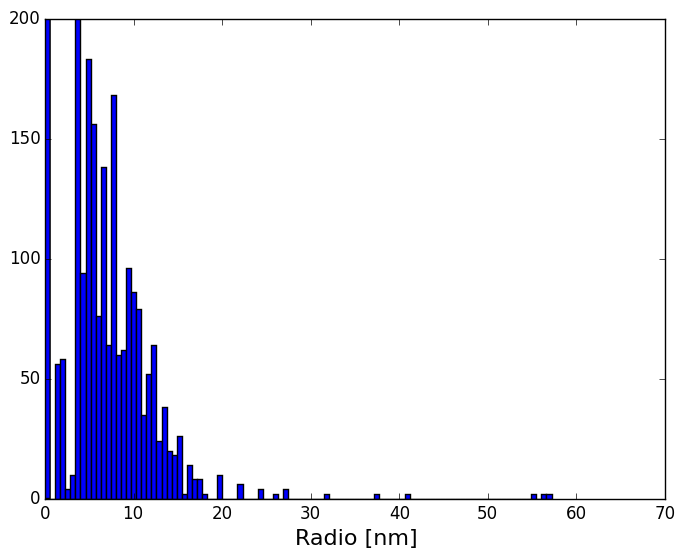
\includegraphics[width=1\linewidth]{poros/160kvm/pulso3}
		\captionof{figure}{Tercer pulso}
		\label{fig:pulso3}
	\end{minipage}%
	\begin{minipage}{.43\paperwidth}
		\centering
		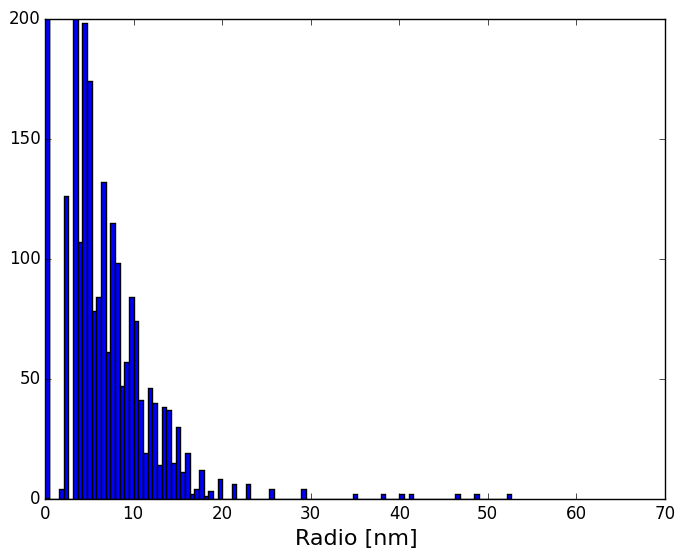
\includegraphics[width=1\linewidth]{poros/160kvm/pulso4}
		\captionof{figure}{Cuarto pulso}
		\label{fig:pulso4}
	\end{minipage}
}
\end{figure}

%TODO conclusiones generales
%TODO mencionar potencial mínimo necesario para electroporación. podría ir tmb un gráfico de itv en tiempo con voltaje bajo sin electroporación
%TODO mencionar que la formula cerrada de itv no sirve
